% Drawing 81/01-4 -- folder 81, batch 01, archive page 10 (PDF page 11).
% Transcription: à droite de « $\mathbb{P}(X)$ » et de « $O\subset\mathbb{P}(X)$ », un croquis à main levée : un petit disque d'où partent des rayons (cinq traits issus de son centre, dont trois dépassent le bord), traversé par une longue droite presque verticale, épaisse au-dessus du centre ; du disque montent des boucles en pétales, et en haut une grande boucle que croisent deux traits obliques.
% Kind: free-hand sketch: small disc with radii, a vertical line and petal loops. Method 2 (schematic redraw from the facsimile). Status: partial.
% Notes: Free-hand ink sketch, redrawn stroke by stroke. The small disc (ellipse) and five strokes from its centre, all drawn from the one centre point: to the upper left and to the upper right (heavy) beyond the rim, to the lower left, to the lower right beyond the rim (hook at its end), and downwards (the continuation of the long line). The long nearly vertical line: thin from the top, heavy from above the disc down to the centre. Loops: a narrow one along the heavy part of the line; a petal from the top of the disc to a tip at the right and back; a tall loop rising from the disc and bending over to the right at the top; an oblique stroke from the line up to the top of that loop; a long oblique stroke falling to the right across the loop, with a short parallel stroke at its end; a small hook and a short curve inside the tall loop; at the right a heavy stroke with a small bar at its top, ending in a hook near the disc. Left out: the letters of « P(X) » that run into the crop at the left. Still differs: the loops are a reading of overlapping free strokes, and their order and joins are approximate; the heavy bottom of the rim is drawn as a heavy arc. The note of the transcription says « aux rayons marqués, d'où partent des boucles en pétales »: agreed. Redrawn 2026-11-10 (issue 128): to check again.
% Coordinates: 1 unit = 1 mm = 1/100 of the crop width (bbox in page fractions: [0.24, 0.12, 0.4, 0.31]).
% Redrawn by Claude (claude-fable-5-2), issue #128, 2026-11-10; not checked by a human; not compiled (no TeX in the session).
% Rights: reproduces part of the work -- behind RENDER_TRANSCRIPTS, never published by itself.
\documentclass[tikz,border=3pt]{standalone}
\usepackage{amsmath,amssymb}
\usetikzlibrary{patterns,arrows.meta}
\tikzset{pencil/.style={black!45}, struck/.style={black!35}, mpt/.style={circle,draw,inner sep=1.3pt}, pt/.style={circle,fill,inner sep=0.9pt}, opt/.style={circle,draw,fill=white,inner sep=1.1pt}}
\begin{document}
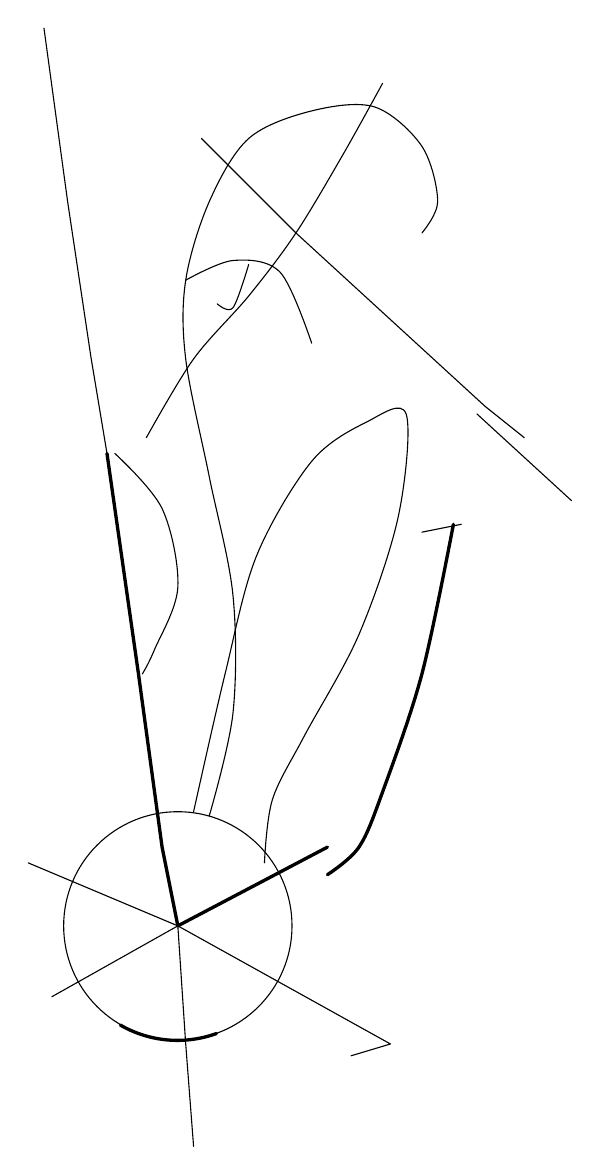
\begin{tikzpicture}[x=1mm,y=1mm,line cap=round,line join=round,font=\scriptsize]
\draw (31,-122) ellipse[x radius=14.5, y radius=14.5];
\draw[very thick] (23.7,-134.6) arc[start angle=240, end angle=290, x radius=14.5, y radius=14.5];
\draw (14,-8) -- (17,-30) -- (20,-50) -- (22,-62);
\draw[very thick] (22,-62) -- (26,-90) -- (29,-112) -- (31,-122);
\draw (31,-122) -- (32,-137) -- (33,-150);
\draw (31,-122) -- (12,-114);
\draw (31,-122) -- (15,-131);
\draw[very thick] (31,-122) -- (50,-112);
\draw (31,-122) -- (58,-137) -- (53,-138.5);
\draw plot[smooth, tension=0.55] coordinates {(23,-62) (29,-69) (31,-79) (28,-87) (26.5,-90)};
\draw plot[smooth, tension=0.55] coordinates {(33,-107.5) (37,-90) (41,-75) (48,-63) (55,-58) (60,-57) (59,-70) (54,-85) (47,-98) (43,-106) (42,-114)};
\draw plot[smooth, tension=0.55] coordinates {(35,-108) (38,-95) (38,-80) (35,-65) (32,-50) (32,-40) (35,-30) (40,-22) (48,-18.5) (56,-18) (62,-23) (64,-30) (62,-34)};
\draw plot[smooth, tension=0.55] coordinates {(27,-60) (33,-50) (40,-42) (46,-34) (52,-24) (57,-15)};
\draw (34,-22) -- (46,-34) -- (70,-56) -- (75,-60);
\draw (69,-57) -- (81,-68);
\draw plot[smooth, tension=0.55] coordinates {(36,-43) (38,-43.5) (40,-38)};
\draw plot[smooth, tension=0.55] coordinates {(32,-40) (38,-37.5) (44,-39) (48,-48)};
\draw (62,-72) -- (67,-71);
\draw[very thick] plot[smooth, tension=0.55] coordinates {(66,-71) (62,-90) (57,-105) (54,-112) (50,-115.5)};
\end{tikzpicture}
\end{document}
